\documentclass[journal=jpclcd,manuscript=suppinfo]{achemso}
\pdfoutput=1
\usepackage{gensymb}
\usepackage{amsmath}
\usepackage{graphicx}
\usepackage{epsfig}
\usepackage{multirow}
\usepackage{multicol}
\usepackage{color}
\renewcommand{\thefigure}{S\arabic{figure}}
% Authors / affiliations
% Authors in alphabetical order except for corresponding author (JJF), need 
% to determine if this is the proper order and if we want to have co-first authors!

\author{Jason Codrington$^{\dagger}$}
\affiliation{Department of Chemistry, William Paterson University, 300 Pompton Road, Wayne, NJ, 07470, USA}
\author{Noor Eldabagh$^{\dagger}$}
\affiliation{Department of Chemistry, William Paterson University, 300 Pompton Road, Wayne, NJ, 07470, USA}
\author{Kimberly Fernando$^{\dagger}$}
\affiliation{Department of Chemistry, William Paterson University, 300 Pompton Road, Wayne, NJ, 07470, USA}
\author{Jonathan J. Foley IV}
\affiliation{Department of Chemistry, William Paterson University, 300 Pompton Road, Wayne, NJ, 07470, USA}
\email{foleyj10@wpunj.edu}

%Title of paper
\title{Supporting Information for Unique hot carrier distributions from scattering mediated absorption}
% Date
\date{\today}


% Being document
\begin{document}

\section{Plots of Global Hot-Carrier Distributions}

\begin{figure}[!ht]
\begin{center}
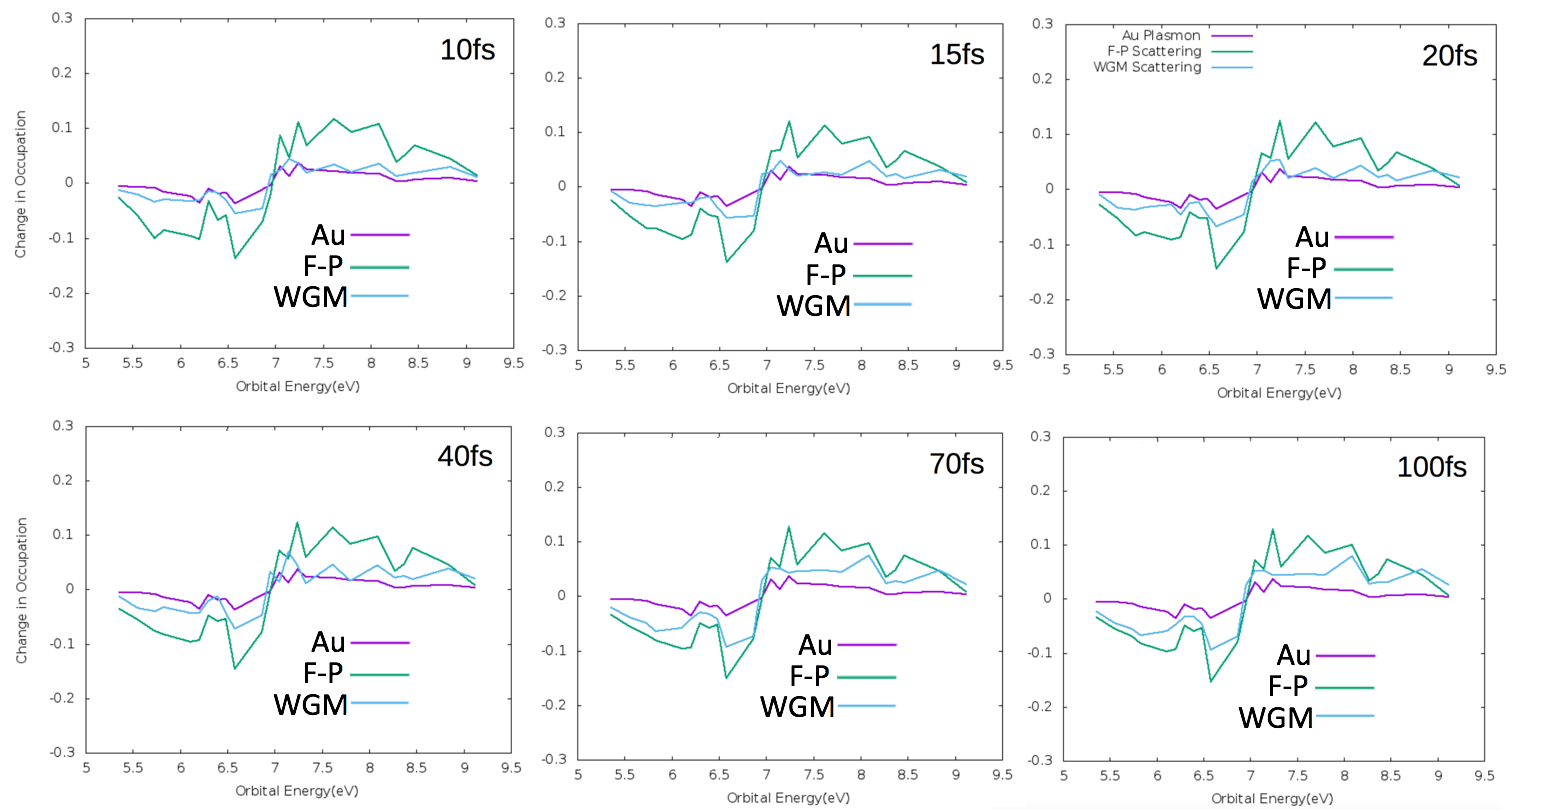
\includegraphics[width=6in]{Au_HotElectronDistribution_Comparison.png}
\caption{Snapshots of changes in occupation of each orbital in the active space of the PIW Au NC model as a measure of instantaneous hot carrier distributions.
The change in orbital occupation is computed from elements of the time-dependent one-electron reduced density matrix ($^1$RDM) relative to
their initial value, $D_p^p(t)-D_p^p(t=0)$ for several timepoints in the simulation.}
\end{center}
\end{figure}


\begin{figure}[!ht]
\begin{center}
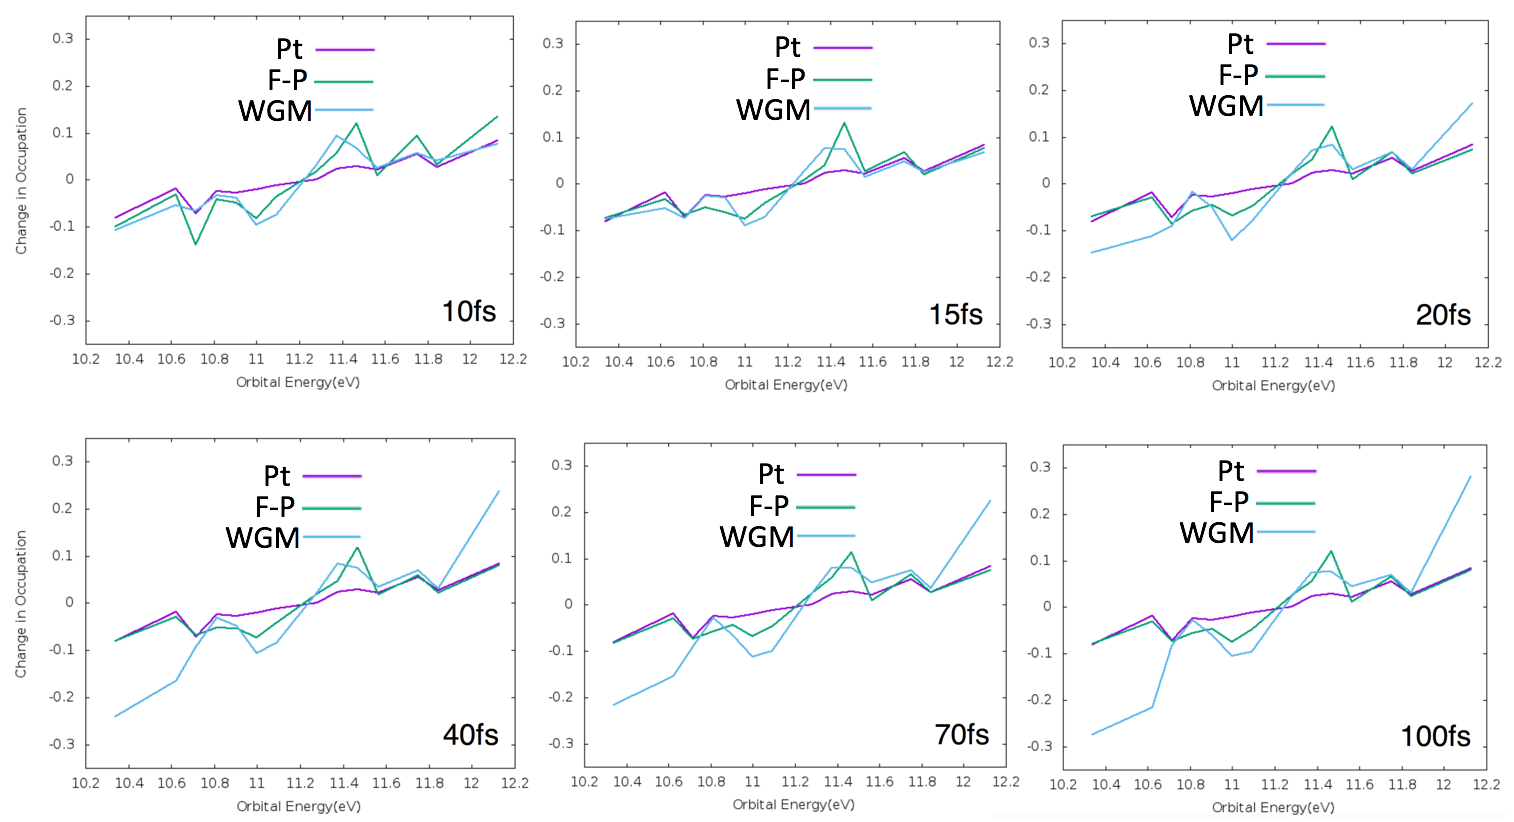
\includegraphics[width=6in]{Pt_HotElectronDistribution_Comparison.png}
\caption{Snapshots of changes in occupation of each orbital in the active space of the PIW Pt NC model as a measure of instantaneous hot carrier distributions.
The change in orbital occupation is computed from elements of the time-dependent one-electron reduced density matrix ($^1$RDM) relative to
their initial value, $D_p^p(t)-D_p^p(t=0)$ for several timepoints in the simulation.  }
\end{center}
\end{figure}


\section{Hot-carrier dynamics in hybrid Ag/dielectric nanostructures}
\begin{figure}
\begin{center}
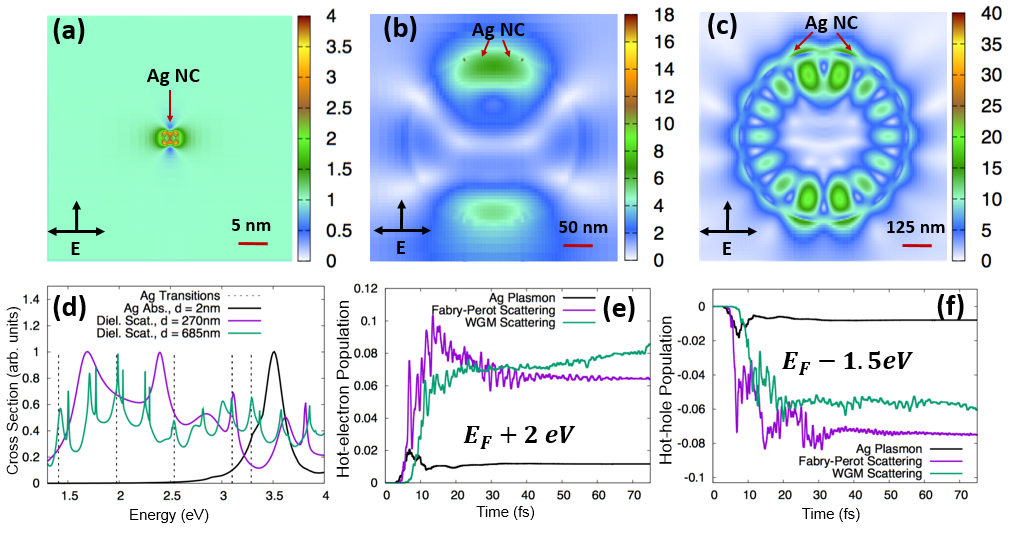
\includegraphics[width=6in]{Ag_AllThree_Revision.png}
\caption{Three regimes for light-matter interactions leading to unique
spatial and temporal shaping of the incident field, and the corresponding
impact on electronic dynamics in a $L=2nm$ PIW Ag nanocube. Plots of the near-field enhancements (${\bf |E|}/{\bf |E_0|}$) are shown for the
Ag NC LSPR ($\lambda=400 nm$, {\bf Panel (a)}), a Fabry-Perot resonance of a d=270nm dielectric nanosphere decorated with Ag NCs ($\lambda = 397 nm$, {\bf Panel (b)}),
and a Whispering Gallery Mode resonance of a d=685 nm dielectric nanosphere decorated with Ag NCs ($\lambda = 493 nm$, {\bf Panel (c)}).
The extinction spectra of these three structures are shown overlaid with the dipole-allowed transitions in the PIW model of the Ag NC, showing 
strong overlap between these transitions and the scattering resonances of the $d=685 nm$ dielectric nanosphere ({\bf Panel (d)}) with only
partial overlap between the Ag LSPR and dipole-allowed transitions in the PIW model.
The change in orbital populations ($D_p^p(t)-D_p^p(t=0)$) is computed to measure hot-electron and hot-hole generation.
Both dielectric scattering resonances show more efficient generation of hot-electrons ({\bf Panel (e)}) and hot-holes ({\bf Panel(f)}) compared to LSPR in this case.}
\end{center}
\end{figure}


\newpage

\section{Electronic structure of metal nanocubes}
For cubic metal nanoparticles, we approximate the one-electron orbitals as energy eigenstates of the particle-in-a-cubic-well.  
For a particle confined by a cubic well with length $L$, the potential is 0 when $x<L, y<L, z<L$ and infinity otherwise.  The energy eigenstates
have the form
\begin{equation}
\psi_{nx,ny,nz} = \left(\frac{2}{L}\right)^{3/2} \: {\rm sin}\left(\frac{n_x \: \pi \: x}{L}\right) {\rm sin}\left(\frac{n_y \: \pi \: y}{L}\right) {\rm sin}\left(\frac{n_z \: \pi \: z}{L}\right).
\end{equation}
The energy eigenvalues have the form
\begin{equation}
\epsilon_{nx,ny,nz} = \frac{\hbar^2 \pi^2}{2 \: m \: L^2}\left(n_x^2 + n_y^2 + n_z^2\right).
\end{equation}
The transition dipole operator can be decomposed into its components,
\begin{equation}
{\bf \hat{\mu} } = \hat{\mu}_x \: {\bf i} + \hat{\mu}_y \: {\bf j} + \hat{\mu}_z \: {\bf k}.
\end{equation}
\textcolor{red}{Given this model, the number of electrons for a given material can be estimated as}
\begin{equation}
N_e = \frac{L^3}{3\pi^2} \left(\frac{2 m E_F}{\hbar^2}   \right)^{3/2}
\end{equation}
\textcolor{red}{where $E_F$ is the experimental Fermi energy for the bulk material of interest.  We assume close-shell systems in all cases and round to the next highest integer value of $N_e$.
Similarly, the Fermi energy in our model can be defined as }
\begin{equation}
E_F^{PIW} = \frac{\hbar^2}{2m} \left(3\pi^2 \frac{N_e}{L^3}  \right)^{2/3},
\end{equation}
\textcolor{red}{where $E_F^{PIW}$ will often be slightly larger than the bulk value of the Fermi energy given that $N_e$ in the above expression
will be rounded to the next highest integer.} 


The transition dipole integral components can be evaluated analytically, for example, the 
$x$-component has the form
\begin{align*}
\langle \psi_{nx,ny,nz} |  \hat{\mu}_x | \psi_{nx',ny',nz'} \rangle = e \: \delta_{ny,ny'} \: \delta_{nz,nz'} \:
\frac{L (\pi (n_x - n_x'){\rm sin}(\pi(n_x - n_x'))+{\rm cos}(\pi(n_x-n_x'))-1) }{\pi^2 (n_x - n_x')^2 } \\
-  e \: \delta_{ny,ny'} \: \delta_{nz,nz'} \:
\frac{L (\pi (n_x + n_x'){\rm sin}(\pi(n_x + n_x'))+{\rm cos}(\pi(n_x+n_x'))-1) }{\pi^2 (n_x + n_x')^2 },
\end{align*}
where $\hat{\mu}_x = -e x$.  Analogous expressions can be obtained for expectation values of $\hat{\mu}_y$ and $\hat{\mu}_z$. 

We order the orbitals by a single index $p$ such that $\epsilon_{p+1} \geq \epsilon_p$; that is,
each $\psi_{nx,ny,nz}$ can be uniquely labeled $\psi_p$.
Using the above expressions and following this labeling scheme, the diagonal matrix elements can be evaluated as
\begin{align}
\langle \Phi_0 | \hat{H}(t) | \Phi_0 \rangle &= \sum_{p=1}^{nocc} \epsilon_p \\
\langle \Phi_i^a | \hat{H}(t) | \Phi_i^a \rangle &= \sum_{p=1}^{nocc} \epsilon_p - \epsilon_i + \epsilon_a
\end{align}
and the off-diagonal matrix elements can be evaluated as
\begin{align}
\langle \Phi_0 | \hat{H}(t) | \Phi_i^a \rangle &=  {\bf E}(t) \cdot \langle \psi_i |  {\bf \hat{\mu}} | \psi_a \rangle \\
\langle \Phi_i^a | \hat{H}(t) | \Phi_j^b \rangle &=   {\bf E}(t) \cdot \langle \psi_a |  {\bf \hat{\mu}} | \psi_b \rangle \delta_{ij}  - {\bf E}(t) \cdot \langle \psi_i | {\bf \hat{\mu}} | \psi_j \rangle \delta_{ab}.
\end{align} 
\textcolor{red}{The precise form of these matrix elements arise because of the antisymmetry 
of the underlying many-electron wavefunction.  It is important to note
that while coulomb repulsion is not included in our current approach, Pauli exclusion, which is
an inherently many-body effect, is enforced by the antisymmetry
of the wavefunction through the Slater-Condon rules used to derive the matrix elements in Eq. (6) through (9).
Importantly, terms analogous to those in Eq. (9) are not included in methodologies like Linear Response Time-Dependent Density
Functional Theory (LR-TDDFT) or methods that use time-dependent perturbation theory (TDPT) to first order.  In fact, setting
the terms in Eq. (9) to zero yields TDPT expressions for the rates of the CIS coefficients.
The terms in Eq. (9) have an important
role in the hot-carrier dynamics in SMA because of the long lifetimes associated with the scattering resonances, and hence, the
long duration of the optical fields that drive these dynamics.  The discrepancy between is shown in Figure S4 where we perform
two calculations with the same driving field: one where the full TDCIS equations are solved, and one where the terms in Eq. (9) 
are set to zero, yielding a equations of motion where only transitions between the ground- and singly-excited
configurations are considered, similar to linear-response or TDPT-based approaches.} 
\begin{figure}
\begin{center}
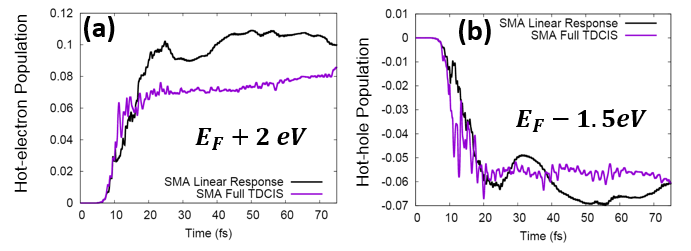
\includegraphics[width=6in]{Ag_LR_vs_TDCIS.png}
\caption{Comparison of hot-electron dynamics as computed from the full TDCIS method and one where
excited-to-excited configurations are neglected in the spirit of approaches based on linear-response
theory and time-dependent perturbation theory to first order.  While the two approaches agree at short
times, the long-time dynamics can show significant departure as population accumulates
in excited-state configurations.  These calculations consider 685 nm dielectric nanospheres (n=2.6)
decorated with 2nm Ag nanocubes. }
\end{center}
\end{figure}


\begin{figure}
\begin{center}
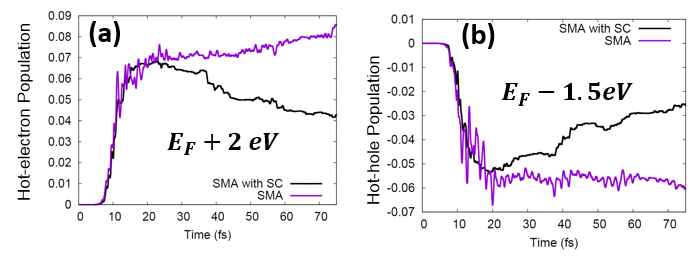
\includegraphics[width=6in]{Ag_SC_Compare.png}
\caption{Comparison of hot-electron dynamics with from SMA with and without a phenomenological size
correction to the dielectric function of silver in 685 dielectric nanospheres (n=2.6) decorated with 2 nm Ag nanocubes.
for Ag-decorated  }
\end{center}
\end{figure}


\section{Finite-difference time-domain calculations}
A commercial simulator based on the finite-difference time-domain method~\cite{Lumerical} was used to compute the electric field, $E(t)$
1 \AA $\:$  
away from the nanoparticle surface in each of the scenarios considered.  The displacement
was taken along the $z$-axis, corresponding to the polarization direction of incident light since the strongest
near-field enhancement is expected along this direction.  A grid spacing of 1 \AA $\:$  
in $x$, $y$, and $z$ was utilized
in a cubic region extending 1 nm beyond the metal NP surface, and a non-uniform mesh was utilized otherwise with $dx$, $dy$, $dz \leq 20 nm$.
For each composite structure, a nanoparticle was placed at the surface of the dielectric nanosphere at an angle of
20$^{\circ}$ with respect to the propagation axis of the incident light. In all simulations, light propagates
along the $x$ axis and is polarized along the $z$ axis.  The metal nanoparticles are centered at $y=0$.  
A total-field scattered-field source was used to illuminate the structures.  The FDTD simulations were terminated when the 
ratio of the total energy in the simulation volume to the total energy injected by the illumination source falls below
$10^{-6}$.  Because the WGMs are higher quality factor resonances, longer time is typically required for these simulations
as compared to the plasmonic particles alone.  

The resulting time-domain fields were fed into our TDCIS algorithm, allowing us to simulate the electronic dynamics
driven by rigorously-computed nearfields from scattering and plasmon resonances, which show strong spatiotemporal modification relative
to freely propagating light.  The electric field was scaled by a factor $E_0 \approx 614,000,000 \: V/m$ so that the peak power
of the illumination source is $10^{15} \: W/m^2$.  The electric field was sampled at intervals of approximately 2.8 attoseconds for all simulations, which leads
to a time-step that ensures stability of
the wavefunction propagation with the relevant energy scales of our simulations.  Our TDCIS scheme
requires the evaluation of the electric field at intermediate times between these timesteps, and we use a simple update
based on centered-finite differences to approximate the electric fields at these times.  As an example, if the 
electric field is known at times $t_1$, $t_2 = t_1 + dt$, and $t_3 = t_1 + 2\cdot dt$ where $dt = 2.8 \: as$, and knowledge
of the field is required at some time $t_m = t_2 + m\cdot dt$ where $m$ is non-integer, $E(t_m)$ is estimated as follows: 
\begin{equation}
{\bf E}(t_m) =  {\bf E}(t_2) + \frac{{\bf E}(t_3)-{\bf E}(t_1) }{t_3 - t_1 } \cdot m\cdot dt.
\end{equation}

The optical response of Au, Pt, and Ag in the FDTD simulations utilizes permittivity 
data from the work of Johnson and Christy~\cite{JC_PRB_1972} (Au) and Palik~\cite{Palik} (Pt and Ag).  
We assume a static dielectric constant of 2.6 for
the dielectric nanospheres in this work, which is comparable to the visible dielectric constant of titanium dioxide. 
\textcolor{red}{The prototype calculation of the impacts on SMA resulting from size effects in the dielectric response
of silver utilizes the phenomenological size correction for the plasmon damping rate in nanocubes suggested by 
Coronado and Schatz~\cite{CS_JCP_2003},}
\begin{equation}
\gamma_{SC} = \gamma_{bulk} + \frac{A v_F}{L_{eff}}
\end{equation}
\textcolor{red}{where $L_{eff} = 2 L/3$ for cubes, where $L$ is 2 nm in this case, we take $A$ to b 1
and $v_F$ is taken to be 1.39e6 $m/s$ for silver.    
We incorporate $\gamma_{SC}$ into a Drude model for the intra-band contribution to silvers dielectric function,}
\begin{equation}
\epsilon_{Drude,SC}(\omega) = 1 - \frac{\omega_P^2}{\omega^2 + i\gamma_{SC}\omega}.
\end{equation}
\textcolor{red}{We take $\omega_P$ and $\gamma_{bulk}$ from a Drude+2Lorentz fit to the Palik data between 200-800 nm;
specifically, $\hbar \omega_P = 8.73 eV$ and $\hbar \gamma_{bulk} = 0.075 eV$.  We infer the
inter-band contribution to the dielectric function from the bulk experimental data and from the bulk Drude fit,}
\begin{equation}
\epsilon_{inter}(\omega) = \epsilon_{Palik}(\omega) - \epsilon_{Drude,bulk}(\omega).
\end{equation}
\textcolor{red}{Finally, the dielectric function used for the size-corrected calculations is defined as}
\begin{equation}
\epsilon_{SC}(\omega) = \epsilon_{inter}(\omega) + \epsilon_{Drude,SC}(\omega).
\end{equation}
\textcolor{red}{Results from these prototpye calculations are shown in Figure S5.}
\bibliography{SMHET_SI} 

\end{document}
   

